%TypeIa.tex
\section{Type Ia Example: 2014J}
The reaction mechanisms of Type Ia supernovae are, like most other supernovae, only gestured at by modern astrophysics; we can guess some of what happens, but the exact mechanisms of the explosion and progenitors remain mysterious. What we do know is that Type Ia lightcurves are remarkably consistent. They have the steepest climb to the &^56&Ni plateau of all the types, post-cooling. We plot this range here for SN2014J: first band by band, then with all the bands compared together.
\begin{figure}
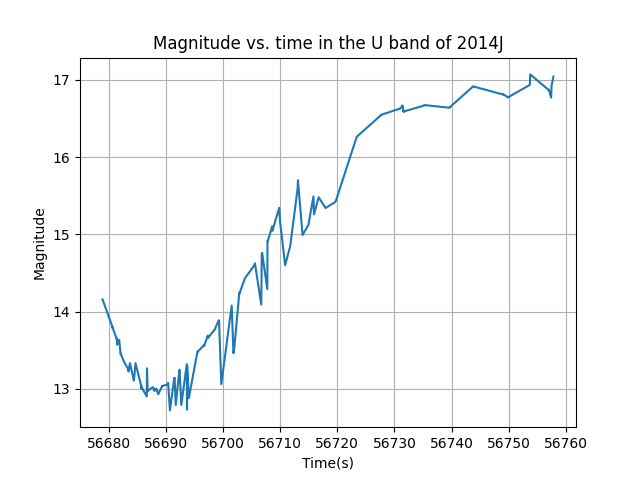
\includegraphics{2014J_U_magvstime.png}
	\caption{Change in brightness of SN2014J across time in the U band.}
\begin{figure}
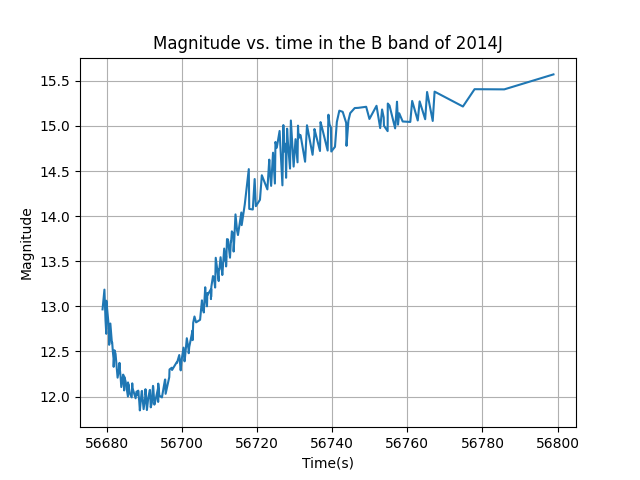
\includegraphics{2014J_B_magvstime.png}
	\caption{Change in brightness of SN2014J across time in the B band.}
\begin{figure}
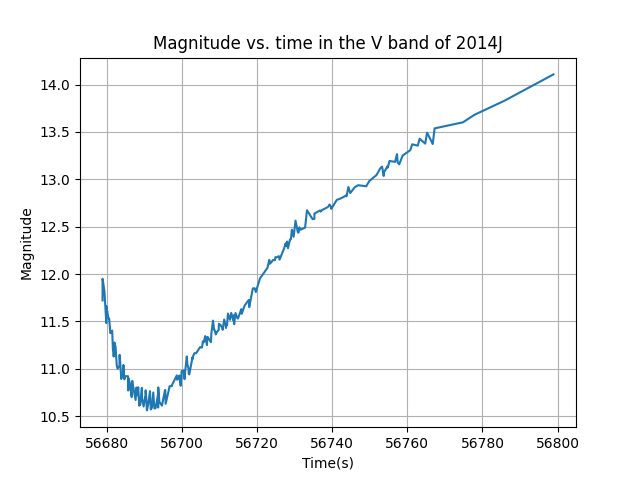
\includegraphics{2014J_V_magvstime.png}
	\caption{Change in brightness of SN2014J across time in the V band.}
\begin{figure}
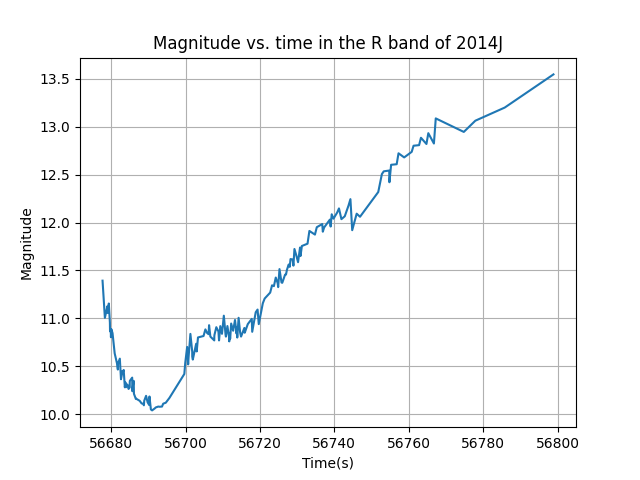
\includegraphics{2014J_R_magvstime.png}
	\caption{Change in brightness of SN2014J across time in the R band.}
\begin{figure}
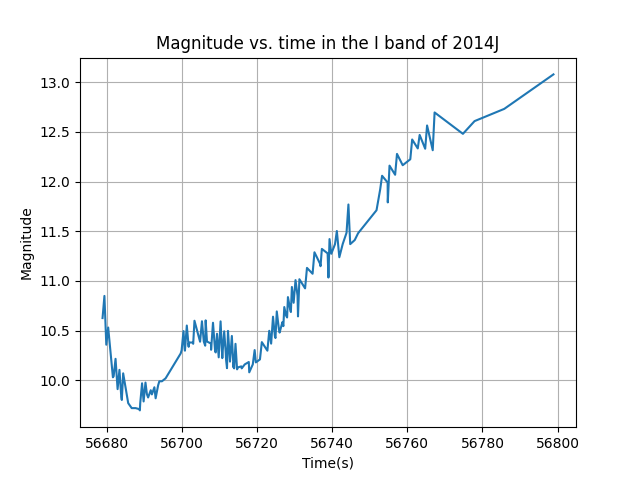
\includegraphics{2014J_I_magvstime.png}
	\caption{Change in brightness of SN2014J aross time in the I band.}

\begin{figure}
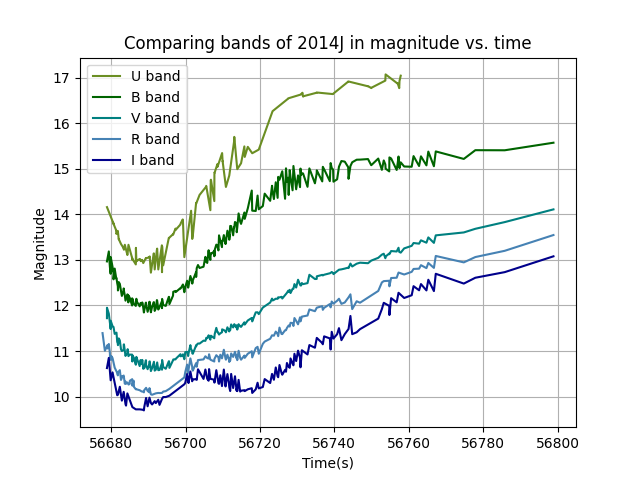
\includegraphics{2014J_all_magvstime.png}
	\caption{All bands of SN2014J together. Note especially the differences between the shape of the I band brightness over time compared to the bluer colors. Just before 56720 seconds, a "shoulder" is visible in the curve. It's beginnings show up in the R band as well.}

